\documentclass[letterpaper]{article}
\title{The Infamous Particle Filter\\16-831 HW3: Fall 2011}
\author{Natasha Kholgade, Heather Knight, and Marynel Vazquez}
\date{}
\usepackage[margin=1in]{geometry}
\usepackage{amsmath}
\usepackage{amssymb}
\usepackage{url}
\usepackage{graphicx}
\usepackage{color}
% Make URL click-able
\usepackage{hyperref}

% Draft for now
%\usepackage{draftwatermark}
%\SetWatermarkLightness{ 0.95 }
%\SetWatermarkScale{ 5 }

% Don't indent after paragraphs
\parindent 0in

\begin{document}

\maketitle

\section{Introduction}

In this assignment, we address the problem of localizing a lost robot within a known map, given its odometry and laser rangefinder data. We implement a particle filter that (1) initializes N particles, (2) uses odometry data to predict the motion model with gaussian noise, (3) uses laser ray casting to assess particle quality based on return probabilities, (4) resamples the particle locations using their weights when the weight variance rises about a threshold. Particle filters are great for situations in which we have sensor and motion data from a known map but no ground truth. We observe good localization performance with a choice of $800$ particles and noise parameters of $\alpha_1=.03, \alpha_2=.03, \alpha_3=.01, \alpha_4=.01$ for the motion model. As the accompanying videos demonstrate, our implementation worked successfully on all of the provided data sets.  

\section{Implementation}

We implement our entire system in MATLAB: the ray casting algorithm is implemented using MEX files, while the rest of the functions are .m files.

\subsection{Particle Initialization}

Given that the dataset depicts a robot traveling through a building, we can assume that the robot was always inside either a room or the hallway.  Thus, we generate our initial samples as a uniform distribution over all pixels that are known but unoccupied with a probability of one (see Fig. \ref{fig1})).  In the next section we use similar reasoning to infer the benefits of discarding (i.e. assign a zero weight to) any particles that go outside the building during the motion modeling.

\begin{figure}[h!tbp]
\centering
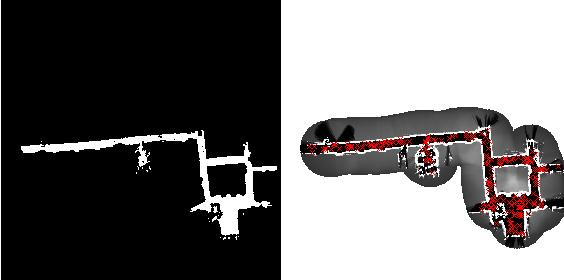
\includegraphics[width=0.8\linewidth]{gen_particles}
\caption[.]{Particle Initialization: (left) map of all pixels that are known but unoccupied 
with a probability of one, (right) full map with initialization with 200 particles}
\label{fig1}
\end{figure}

\subsection{Motion Model}

We use the motion model described in Thrun et al. [1] in this assignment. Our motion model uses the odometry data only to estimate the motion relative to the current particle frames, also incorporating Gaussian noise to model the presence of inaccuracies in the odometry sensing more robustly, as depicted in our motion model testing images in Fig. \ref{fig2}).

\begin{figure}[h!tbp]
\centering
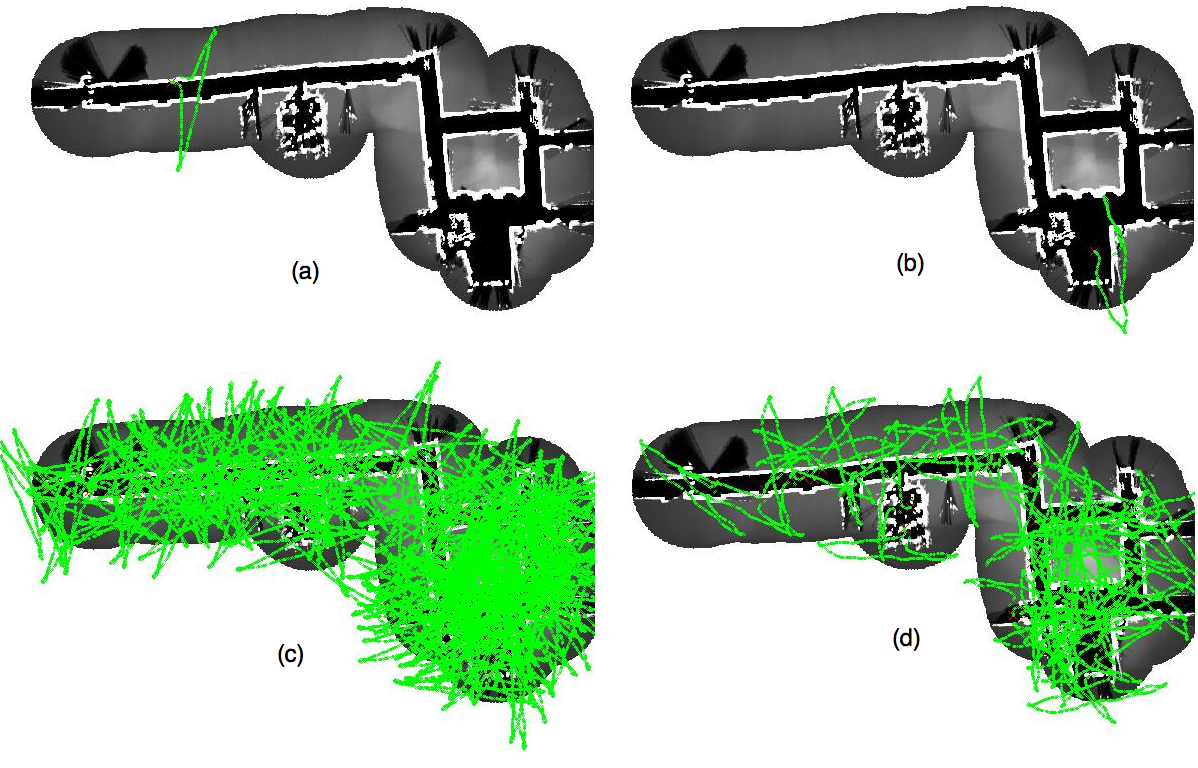
\includegraphics[width=0.8\linewidth]{all_motionmodel}
\caption[.]{Motion Model without Sensor model for (a) one particle with no noise, 
(b) one particle with noise, (c) 200 particles no noise, (d) 200 particles with noise
}
\label{fig2}
\end{figure}
\subsubsection{The Motion Equations}

To get motion estimates from one odometry configuration $(\tilde{x},\tilde{y},\tilde{\theta})$ to another $(\tilde{x}',\tilde{y}',\tilde{\theta}')$ on a two dimensional plane, the robot needs to perform a rotation to align with the direction of travel, a translation along that direction, and a rotation to adjust itself to the final orientation (Figure \ref{fig3}). 

\begin{figure}[h!tbp]
\centering
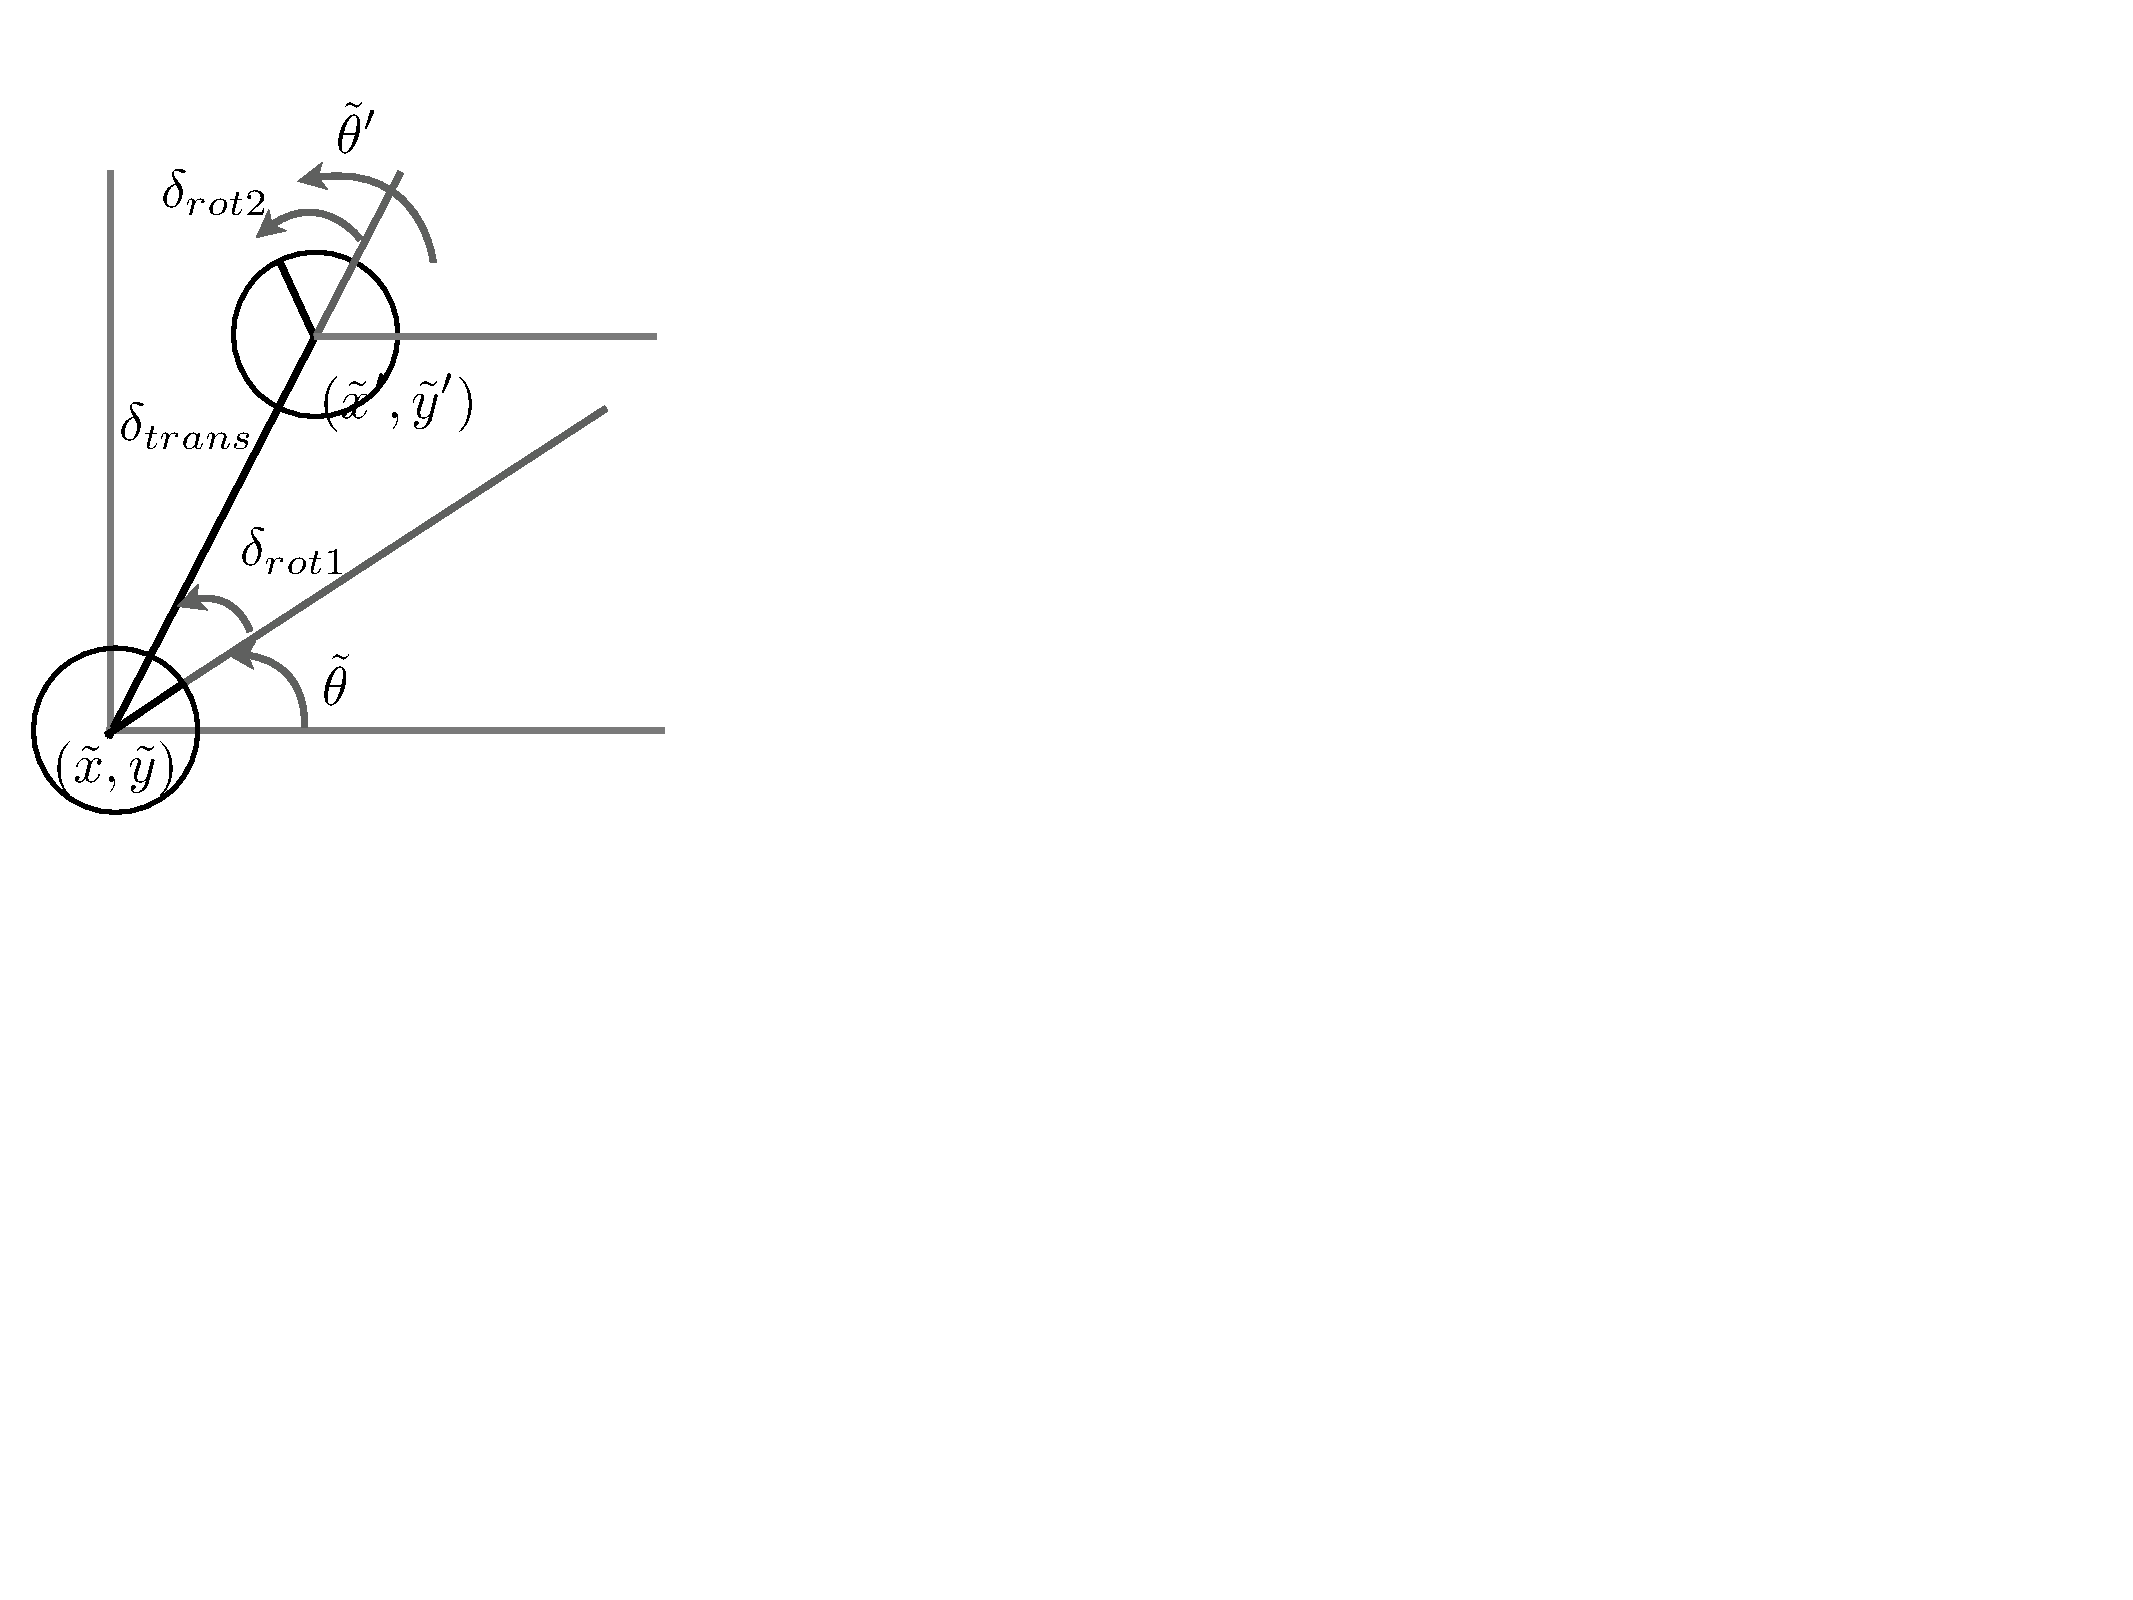
\includegraphics[width=.3\linewidth]{motionmodel}
\caption[.]{Motion model for a robot moving from configuration $(\tilde{x},\tilde{y},\tilde{\theta}$ to $(\tilde{x}',\tilde{y}',\tilde{\theta}')$}
\label{fig3}
\end{figure}

The initial change in rotation can be specified as:
$$\delta_{rot1}=\text{atan2}(\tilde{y}'-\tilde{y},\tilde{x}'-\tilde{x})-\tilde{\theta}$$
The change in translation is the distance travelled between the initial and final locations:
$$\delta_{trans}=\sqrt{(\tilde{x}'-\tilde{x})^2+(\tilde{y}'-\tilde{y})^2}$$
The final change in rotation is given as
$$\delta_{rot2}=\tilde{\theta}'-\tilde{\theta}-\delta_{rot1}$$

\subsubsection{Incorporating Noise}
We assume that the actual values of rotation and translation can be described by removing independent noise $\epsilon_b$ with zero mean and variance $b$:
$$ \hat{\delta}_{rot1}=\delta_{rot1}-\epsilon_{\alpha_1 \left|\delta_{rot1}\right|+\alpha_2 \left|\delta_{trans}\right|}$$
$$ \hat{\delta}_{trans}=\delta_{trans}-\epsilon_{\alpha_3 \left|\delta_{trans}\right|+\alpha_4 \left|\delta_{rot1}+\delta_{rot2}\right|}$$
$$ \hat{\delta}_{rot2}=\delta_{rot2}-\epsilon_{\alpha_1 \left|\delta_{rot2}\right|+\alpha_2 \left|\delta_{trans}\right|}$$
The updates to the translation and rotation are given by:
$$x'=x+\hat{\delta}_{trans}\cos(\theta+\hat{\delta}_{rot1})$$
$$y'=y+\hat{\delta}_{trans}\sin(\theta+\hat{\delta}_{rot1})$$
$$\theta'=\theta+\hat{\delta}_{rot1}+\hat{\delta}_{rot2}$$

\subsubsection{Sampling Distribution}

We obtain all our samples from a normal distribution centered around the quantity of interest:

$$x \sim \mathcal{N}(\overline{x}, \sqrt{b})$$

To obtain a random sample according to the normal distribution, we randomly generate a set of $12$ values from the uniform distribution between -1 and 1, sum them, and multiply by the factor $b/6$ where $b$ is the variance of the distribution.

\subsubsection{Training the $\alpha's$}

We found that having larger noise for the rotation parameters $\alpha_1$ and $\alpha_2$ versus the translation parameters $\alpha_3$ and $\alpha_4$ was important.  The rotation space for all possible $\alpha's$ given the number of particles we have is very large, thus we found small rotation parameters made it unlikely that our particles would happen to be at the best orientations. Small horizontal and vertical translation errors were easier to recover from by comparison.

\subsubsection{Validation}

We tested the motion model individually before integration. In the first example, we generated a single particle and ran the the motion model without noise to ensure its motion mimicked the motion from the odometry data. Next we evaluated a many particles with noise but no sensor or resampling feedback. Contrasting the many particles with noise case in Fig. 2 to that without, you see how an enough particles can be resilient against inaccuracies in the odometry data because there are variations in the particle actions. One sees this even better by initializing a bunch of particles to the same starting point and observing the spread. When a satisfactory banana-shaped spread was obtained, we moved on to the next step.

\subsection{Sensor Model}

\begin{figure}[t]
\centering
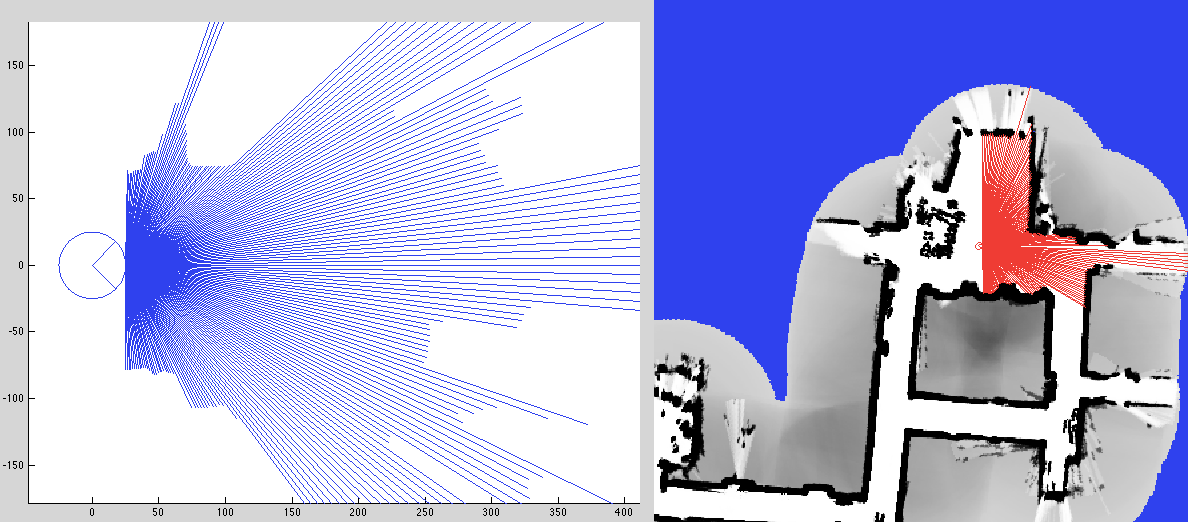
\includegraphics[width=.9\linewidth]{laser}
\caption[.]{Visualizing Laser Data in action: (left) Model of robot with laser location displaced from center, (right) Displaying beams interpolated onto the true map}
\label{fig4}
\end{figure}

We actually implemented four different methods for assessing the sensor model. We have a simple probabilistic map model in which we summed and exponentiated the probabilities of each expected hit point over each particle's rays. Next we thresholded the hits to zero or one and counted the total hits per particle. After limited success with the simple model, we elected to implement ray tracing, first in Matlab and then in C++. To ensure the overall solution would consistently converge, there were also several pre-processing steps that were important to implement carefully. \\ 

The original sampling of the environment by the sensor data was highly non-uniform. In particular, there were a large number of points in close proximity to the robot and fewer points far from the robot.  If the likelihood was calculated over all of these data points, the information carried by points farther away would be overshadowed by the large quantity of near points. In addition, the laser itself has a max range, and so there are frequent artificial peaks at 8000cm. To remedy these problems, we filtered the points along the path of the ray. 

\subsubsection{Simple Probabalistic Map Model}

When an observation is made, the laser data is projected into the smoothed map from each particle location.  In our first model, the sensor model assumes independence between all laser points so the likelihood of a scan is taken to be the product of the likelihoods of each of the individual points. (Note that the laser on the robot is approximately 25 cm offset forward from  the true center of the robot.) The likelihood of each ray containing a successful hit is computed as a mixture of a normal and a uniform distribution: 
$$Lpoint = z_{hit} * prob(dist, \sigma_{hit}) + z_{uniform} $$

The above $z�s$ are the weights used in mixing the distributions and $prob(dist, \sigma_{hit})$ computes the probability of the distance to the nearest obstacle under a zero-mean Gaussian distribution with standard deviation $\sigma_{hit}$. The $z_{uniform}$ term allows for the rejection of noise at the cost of slowing down convergence. 

Note that we smooth the map beforehand to improve results but this smoothing is not performed at each time step, as that would increase computation significantly. Instead the map can be smoothed once for all  particles at the beginning of the particle filter.

\subsubsection{Raytracing Model}

Raytracing computes $P(x|z)$ by ray casting beams and comparing hits in the map with laser measurements. The probability for a hit is computed using a normal distribution centered at the laser measurement for a beam (with $\sigma = \sigma_{beam}$).  First we filter the beams that do not meet the minimum and max thresholds. Next, we cast the ray linearly out from the particle location, ensuring that the hit characteristics occur at the first object or wall encountered rather than giving a false positive for an obstructed feature that its lasers would not be able to sense. Given this data over all possible particle rays (literally 180 beams, although we subsample by a factor of four).

\subsubsection{Computing Weights}

Weights using the probabilities from the map-based sensor model: $W = sum(hitProb)$ \\

Weights counting thresholded probabilities from map: $W = sum(hitProb > 0.8)+epsilon$ \\

Weights from ray casting: $W = exp(sum(probs,2))$ 

\subsubsection{Validation}

It took many steps to integrate our sensor model into the overall particle filter, but before that we isolated the functioning of the Sensor Model itself by creating a point and click interface to insert oriented particles into the map and estimate the rays from that center.  Other steps we used to validate its functioning included A, B and C. [FEEL FREE TO ELABORATE]\\

Once we were confident in the sensor model itself, integrating this step into the overall particle filtering functioning involved many iterations of parameter testing. Challenged we faced were choosing how often to resample (discussed in the next section), evaluating $\alpha$ values, and matching up coordinate systems across the code of the various project contributors.

\subsection{Resampling Step}

As discussed in class, we used Normalized Importance Resampling to redistribute the particles over the previous particle space in a manner that reflects their overall probability levels as expressed by the particles� most recent weights.  

\subsubsection{Methodology}
Specifically, for the $N$ particles we create $N$ bin indices by using their weights to create a continuous PDF. We accomplish that by creating a cumulative sum of weights for each sequential particle, then dividing each by the sum of all possible weights. Next, we generate a random number between zero and one as the first resampling position, using the continuous PDF index of that location to assign the first particle in our new set of particles. After that we iterate $N-1$ times, moving our sampling position forward by $1/N$ with a circular buffer. When resampling is complete, we match our new particles with the stored indices and reset all weights.

\subsubsection{Resampling Frequency}
We do not resample the particles at explicit timestep, but rather track the overall variance in the weights and only perform resampling when the variance of weights has surpassed a certain threshold. We experimentally determining a good variance threshold by tracking how long it took unlikely particles or particle clusters to die out, while maintaining enough diversity in the particle distribution to allow reliable convergence. \\

 Resampling too often can lead to lack of particle diversity and thus loss of information, not resampling enough means the algorithm will not converge and means fewer additional particles will be added to the true particle location, which could make that true particle location less robust to noise.

\section{Algorithm Summary}

Our particle filter code consists of the following:

\begin{verbatim}
Initialization:
_ 1. Generate N particles using a uniform distribution over the valid positions in the map and all
_ possible headings. 
_ 2. Smooth our map by convolving it with a gaussian.

While there is still data:
_ If weights variance above threshold:
___ 1. Resample particles
___ 2. Set new particle weights to 1/N
_ If next reading is Odometry:
___ 1. Use the motion model to predict the next particle location.
___ 2. Throw out any particle that goes off the map.
_ If next reading is Laser data:
___ 1. Use the motion model to forward simulate where each particle would be at the time 
___ of the scan.
___ 2. Filter the laser data as described above.
___ 3. Project the sensor data into the world using the particle�s position and heading and 	
___ use the likelihood field to compute a weight for each particle.
___ 4. Sample a new batch of particles using the distribution of the weights to sample from 	
___ the old set of particles.
\end{verbatim}

It also generates the map and sensor visualization for each step along the way.

\section{Results}

[ADD PICTURE FRAME FROM ONE OF THE FINAL SUCCESSFUL VIDEOS]\\
 
As the accompanying videos demonstrate, our implementation worked successfully on all of the provided data sets.  Note: to execute our accompanying code, use the function: 
$$runParticleFilter(map, dataLogName, desiredNumberParticles)$$

As the movies show, our particle filter algorithm converges to the correct global position after around 200 iterations. We used 800 particles, which we depict as blue dots. For the highest likelihood particle,  we plot an oriented circle with triangle depicting laser location and use its pose to transform the filtered laser data into red beams in the world coordinates. If the filter is working properly, its laser readings should align with map obstacles. 

\section*{References}

[1] Thrun, S., Burgard, W., and Fox, D. \emph{Probabilistic Robotics}, The MIT Press, 2005. 

\end{document}
